\documentclass[aspectratio=43]{beamer}
% aspectratio=1610,169

\usepackage[czech]{babel}
\usepackage[utf8]{inputenc}
\usepackage[T1]{fontenc}
\usetheme[workplace=sci,]{MU}
\usepackage{tikz}
\usepackage{scalerel}
\usepackage{tcolorbox}
\usepackage{xcolor}
\usepackage{bbding}
\usepackage{pifont}
\usepackage{wasysym}
\usepackage{amssymb}
\usepackage{rotating}

\definecolor{myblack}{RGB}{27,27,27}
\definecolor{mycolor}{RGB}{255,255,255}
\definecolor{myblue}{RGB}{95,120,219}
\definecolor{limegreen}{RGB}{164,244,207}

\newcommand{\myarrow}[1][0.1pt]{\tikz[baseline=-0.26em,y=3em, x=3em]{\filldraw[line width=#1] (0.4202,0.0021) .. controls (0.4202,-0.0000) and (0.4188,-0.0018) .. (0.4171,-0.0025) .. controls (0.3917,-0.0092) and (0.3699,-0.0236) .. (0.3509,-0.0401) .. controls (0.3355,-0.0538) and (0.3225,-0.0704) .. (0.3130,-0.0890) .. controls (0.3119,-0.0915) and (0.3094,-0.0929) .. (0.3066,-0.0929) .. controls (0.3028,-0.0929) and (0.2996,-0.0897) .. (0.2996,-0.0858) .. controls (0.2996,-0.0848) and (0.3000,-0.0837) .. (0.3003,-0.0827) .. controls (0.3087,-0.0665) and (0.3193,-0.0517) .. (0.3316,-0.0391) -- (0.1181,-0.0391) .. controls (0.1143,-0.0391) and (0.1111,-0.0359) .. (0.1111,-0.0320) .. controls (0.1111,-0.0282) and (0.1143,-0.0250) .. (0.1181,-0.0250) -- (0.3471,-0.0250) .. controls (0.3611,-0.0137) and (0.3766,-0.0046) .. (0.3935,0.0021) .. controls (0.3766,0.0088) and (0.3611,0.0179) .. (0.3471,0.0292) -- (0.1181,0.0292) .. controls (0.1143,0.0292) and (0.1111,0.0323) .. (0.1111,0.0362) .. controls (0.1111,0.0401) and (0.1143,0.0432) .. (0.1181,0.0432) -- (0.3316,0.0432) .. controls (0.3193,0.0559) and (0.3087,0.0707) .. (0.3003,0.0868) .. controls (0.3000,0.0879) and (0.2996,0.0889) .. (0.2996,0.0900) .. controls (0.2996,0.0939) and (0.3028,0.0970) .. (0.3066,0.0970) .. controls (0.3094,0.0970) and (0.3119,0.0956) .. (0.3130,0.0932) .. controls (0.3225,0.0745) and (0.3355,0.0580) .. (0.3509,0.0443) .. controls (0.3699,0.0278) and (0.3917,0.0133) .. (0.4171,0.0067) .. controls (0.4188,0.0059) and (0.4202,0.0042) .. (0.4202,0.0021) -- cycle;}}

\setbeamertemplate{sidebar right}{}
\setbeamertemplate{footline}{\bf \begin{flushright}\insertframenumber{}$\,$/$\,$\inserttotalframenumber \hphantom{aaaa.}\end{flushright}\vspace{-0.11cm}}

\setbeamercolor{normal text}{fg=white,bg=myblack}
\useoutertheme[subsection=false]{miniframes}

\newcommand{\OPACITY}{0.6}

\begin{document}

\begin{frame}[noframenumbering,plain]
\begin{tikzpicture}[overlay]
    \draw (5.675, -5) node[opacity=0.6] {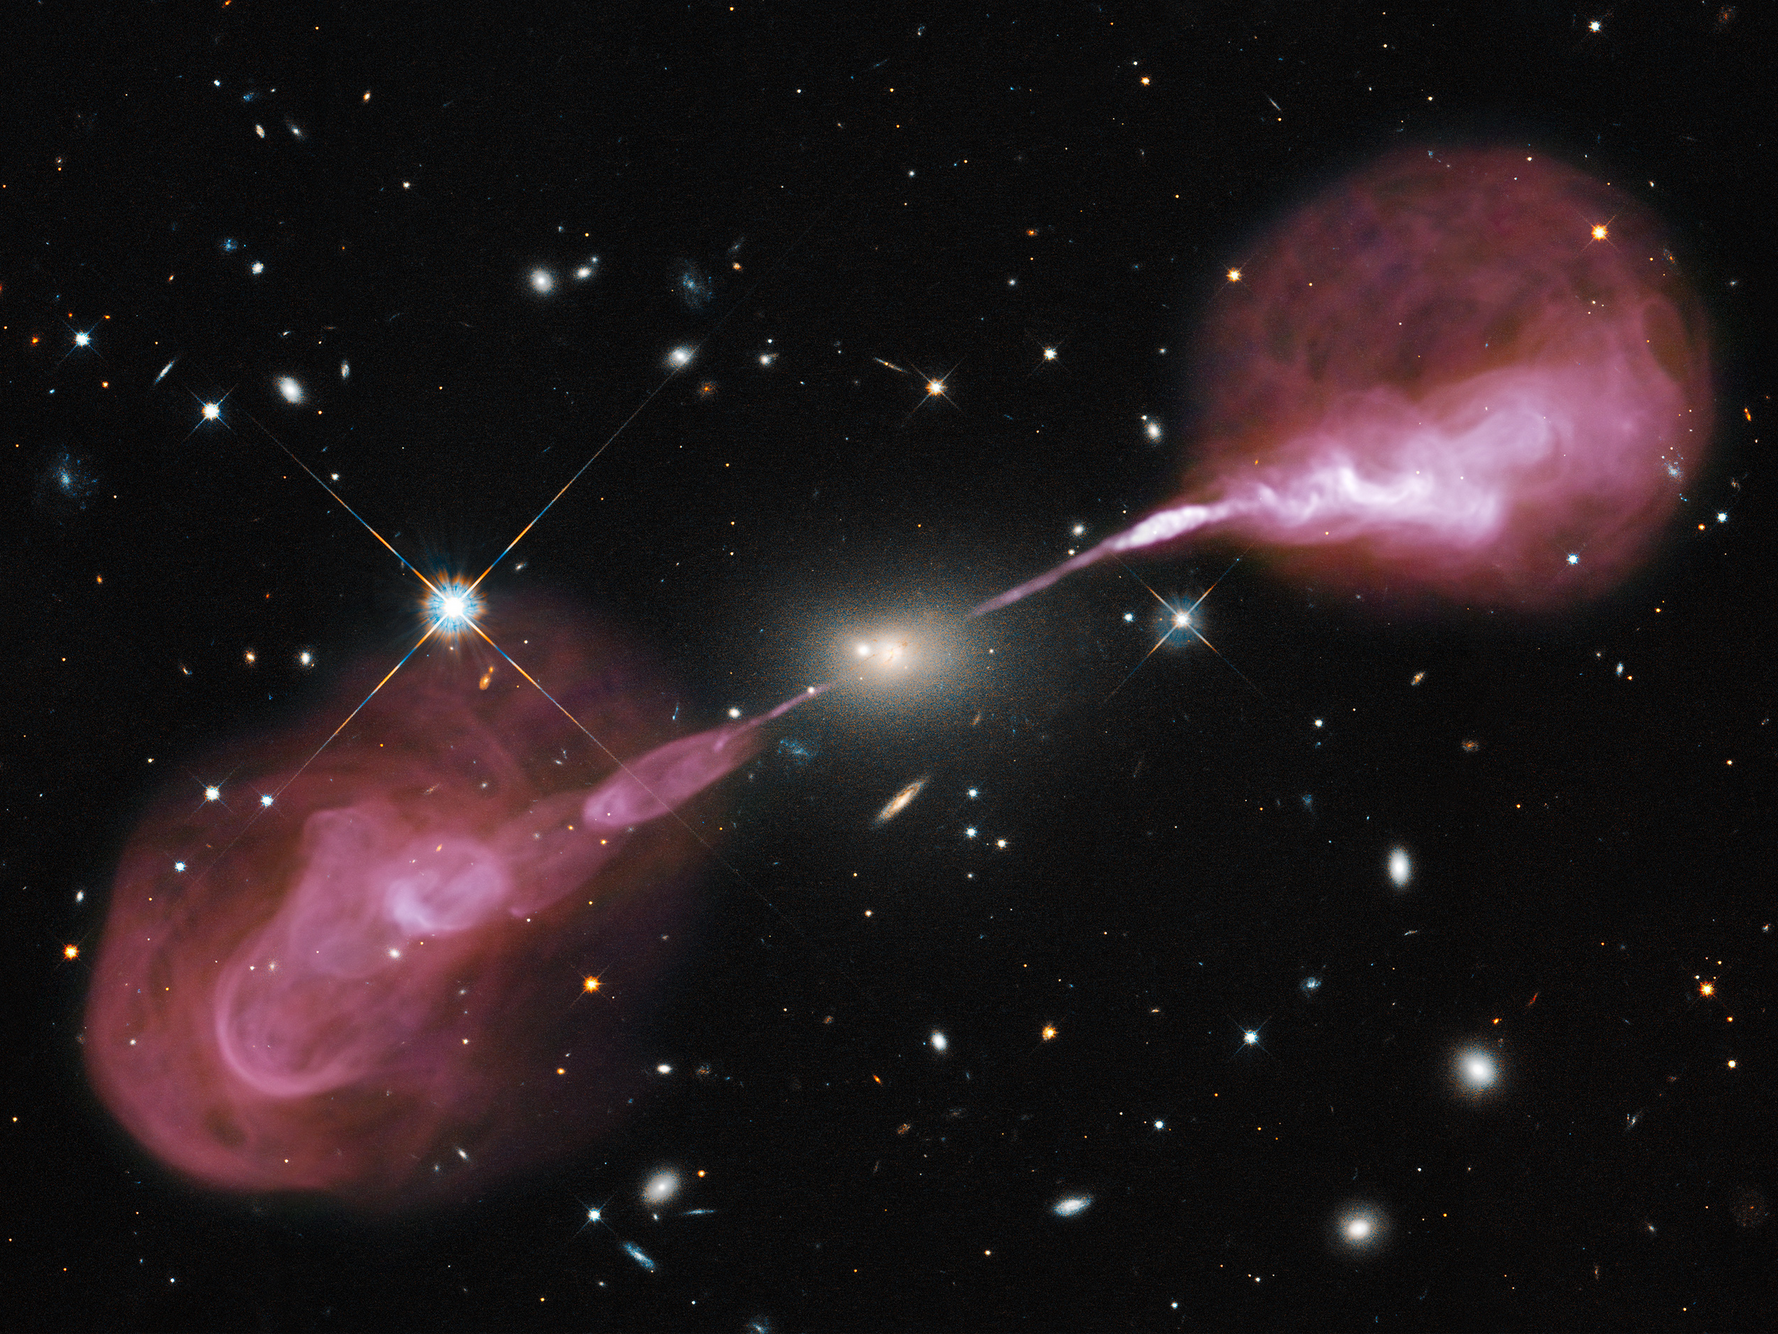
\includegraphics[width=400pt]{figures/hercules_A_flop.png}};

    \draw (10.6, -1.33) node {\includegraphics[height=42pt]{mubeamer/logo/mubeamer-sci-english-color.png}};
    % \draw[fill=myblack,myblack] (7.4,-2.1) rectangle (9.8,-0.2);
    % \draw (6.80, -1.27) node {\includegraphics[height=45pt]{mubeamer/logo/mubeamer-sci-english-color.pdf}};

    \draw (2.15, -1.27) node {\includegraphics[height=30pt]{mubeamer/label/mubeamer-mu-english-color.pdf}};
    % \draw (10.35, -1.30) node {\includegraphics[height=55pt]{CADET/CADET.png}};

    \draw (5.675, -4.3) node {\Huge \bf Mechanická zpětná vazba};
    \draw (5.675, -5.6) node {\Huge \bf aktivích galaktických jader};
    % \draw (5.675, -5.9) node {\includegraphics[width=300pt]{CADET/blocks_2.png}};

    \draw (-0.05, -8.92) node[right] {\large \bf Tomáš Plšek};
    \draw (5.60, -8.92) node {\large Astronomická expedice};
    \draw (11.45, -8.92) node[left] {\large 4. sprna 2022};
\end{tikzpicture}
\vspace{105mm}
\end{frame}

\begin{frame}[noframenumbering,plain]{\vspace{-2mm}High Energy Astrophysics group\phantom{j$^1$}\\\vspace{1.5mm}\hrule}
\vspace{8mm}
\begin{itemize}
    \item<2-8> Přírodovědecká Fakulta, MUNI, Brno\\ \vspace{3mm}
        -- budova 8, Kotlářská 2, Brno\\ \vspace{5mm}
    \item<3-8> Vedoucí skupiny: prof. Norbert Werner\\ \vspace{5mm}
    \item<4-8> zaměření:\\ \vspace{3mm}
        -- výzkum horkého vesmíru\\ \vspace{3mm}
        -- aplikace strojového učení\\ \vspace{3mm}
        -- detekce GRB pomocí nanosatelitů\\ \vspace{3mm}
        -- český UV teleskop (QUVIK)\\
\end{itemize}
\begin{tikzpicture}[overlay]
    \draw<1> (5.7, 4.0) node  {\includegraphics[height=180pt]{figures/team.jpg}};

    \draw<2-8> (5.7, 7.55) node {\url{hea.physics.muni.cz}};
    \draw<2-8> (10.3, 7.0) node {\includegraphics[height=45pt]{figures/kotlarska.jpg}};
    \draw<3-8> (10.3, 4.95) node {\includegraphics[height=56pt]{figures/norbert.jpg}};
    \draw<5-8> (7.34, 3.25) node {\includegraphics[height=45pt]{figures/hea.jpg}};
    \draw<6-8> (9.9, 2.7) node {\includegraphics[height=45pt]{figures/astro_AI.jpg}};
    \draw<7-8> (7.9, 1.45) node {\includegraphics[height=45pt]{figures/grbalpha.jpg}};
    \draw<8> (9.75, 0.9) node {\includegraphics[height=45pt]{figures/quvik.png}};
\end{tikzpicture}
\end{frame}

\begin{frame}{\vspace{-2mm}Obsah\phantom{j$^1$}\\\vspace{1.5mm}\hrule}
\large \bf
\begin{tikzpicture}[overlay]
    \draw<2-> (10.2, 1.7) node {\includegraphics[height=31pt]{figures/elipsa.png}};
    \draw<3-> (8.2, 0.2) node {\includegraphics[height=43pt]{figures/AGN.png}};
    \draw<4-> (10.2, -1.3) node {\includegraphics[height=43pt]{figures/loby.png}};
    \draw<5-> (8.2, -2.8) node {\includegraphics[height=40pt]{figures/blackcadet.png}};

    \draw<1> (0.1, 1.7) node[right,opacity=\OPACITY] {$\bullet\;\;$ Galaxie raného typu\vspace{8.0mm}};
    \draw<1> (0.1, 0.2) node[right,opacity=\OPACITY] {$\bullet\;\;$ Aktivní galaktická jádra (AGN)\vspace{8.0mm}};
    \draw<1> (0.1, -1.3) node[right,opacity=\OPACITY] {$\bullet\;\;$ Zpětná vazba AGN\vspace{8.0mm}};
    \draw<1> (0.1, -2.8) node[right,opacity=\OPACITY] {$\bullet\;\;$ Cavity Detection Tool (CADET)};

    \draw<2> (0.1, 1.7) node[right] {$\bullet\;\;$ Galaxie raného typu\vspace{8.0mm}};
    \draw<2> (0.1, 0.2) node[right,opacity=\OPACITY] {$\bullet\;\;$ Aktivní galaktická jádra (AGN)\vspace{8.0mm}};
    \draw<2> (0.1, -1.3) node[right,opacity=\OPACITY] {$\bullet\;\;$ Zpětná vazba AGN\vspace{8.0mm}};
    \draw<2> (0.1, -2.8) node[right,opacity=\OPACITY] {$\bullet\;\;$ Cavity Detection Tool (CADET)};

    \draw<3> (0.1, 1.7) node[right,opacity=\OPACITY] {$\bullet\;\;$ Galaxie raného typu\vspace{8.0mm}};
    \draw<3> (0.1, 0.2) node[right] {$\bullet\;\;$ Aktivní galaktická jádra (AGN)\vspace{8.0mm}};
    \draw<3> (0.1, -1.3) node[right,opacity=\OPACITY] {$\bullet\;\;$ Zpětná vazba AGN\vspace{8.0mm}};
    \draw<3> (0.1, -2.8) node[right,opacity=\OPACITY] {$\bullet\;\;$ Cavity Detection Tool (CADET)};

    \draw<4> (0.1, 1.7) node[right,opacity=\OPACITY] {$\bullet\;\;$ Galaxie raného typu\vspace{8.0mm}};
    \draw<4> (0.1, 0.2) node[right,opacity=\OPACITY] {$\bullet\;\;$ Aktivní galaktická jádra (AGN)\vspace{8.0mm}};
    \draw<4> (0.1, -1.3) node[right] {$\bullet\;\;$ Zpětná vazba AGN\vspace{8.0mm}};
    \draw<4> (0.1, -2.8) node[right,opacity=\OPACITY] {$\bullet\;\;$ Cavity Detection Tool (CADET)};

    \draw<5> (0.1, 1.7) node[right,opacity=\OPACITY] {$\bullet\;\;$ Galaxie raného typu\vspace{8.0mm}};
    \draw<5> (0.1, 0.2) node[right,opacity=\OPACITY] {$\bullet\;\;$ Aktivní galaktická jádra (AGN)\vspace{8.0mm}};
    \draw<5> (0.1, -1.3) node[right,opacity=\OPACITY] {$\bullet\;\;$ Zpětná vazba AGN\vspace{8.0mm}};
    \draw<5> (0.1, -2.8) node[right] {$\bullet\;\;$ Cavity Detection Tool (CADET)};
\end{tikzpicture}
\end{frame}


\section{Galaxie raného typu}

\begin{frame}{\vspace{-2mm}Rozdělení galaxií\phantom{j$^1$}\\\vspace{1.5mm}\hrule}
\begin{tikzpicture}[overlay]
    % \draw<1-> (10.75, 3.65) node {\includegraphics[height=22pt]{figures/elipsa.png}};
    \draw<1-> (5.7, -0.6) node {\includegraphics[height=190pt]{figures/hubble.png}};
    \draw<2>[color=white,thick] (3.5,-0.47) ellipse (2cm and 1.6cm);
\end{tikzpicture}
\end{frame}

\begin{frame}{\vspace{-2mm}Galaxie raného typu\phantom{j$^1$}\\\vspace{1.5mm}\hrule}
\vspace{-0.2mm}
\begin{itemize}
    \item<1->[\color{white}=] eliptické a čočkové galaxie\\ \vspace{3.0mm}
    \item<2-> označení "red \& dead"\\ \vspace{1.4mm}
        -- staré chladnější hvězdy\\ \vspace{1.4mm}
        -- nízká tvorba nových hvězd\\ \vspace{3.0mm}
    \item<3-> poblíž kup galaxií\\ \vspace{3.0mm}
    \item<4-> systémy s $\;\text{M}$ > $10^{12} \; \text{M}_{\odot}$\\ \vspace{1.5mm}
        -- aktivní galaktická jádra\\ \vspace{1.5mm}
        -- horké atmosféry\\ \vspace{3.5mm}
\end{itemize}
\begin{tikzpicture}[overlay]
    % \draw<1-> (10.75, 7.34) node {\includegraphics[height=22pt]{figures/elipsa.png}};
    \draw<1-3> (8.25, 4.65) node {\includegraphics[width=110pt]{figures/elliptical_1.jpg}};
    \draw<1-3> (8.25, 0.90) node {\includegraphics[width=110pt]{figures/lenticular_1.jpg}};
    \draw<3> (2.90, 0.90) node {\includegraphics[width=155pt]{figures/galaxy_cluster.jpeg}};
    % \draw<4> (8.6, 2.9) node {\includegraphics[height=150pt]{figures/M87.png}};
    \draw<4> (8.5, 3.2) node {\includegraphics[height=130pt]{figures/schema.png}};
\end{tikzpicture}
\end{frame}

\begin{frame}{\vspace{-2mm}Horké atmosféry\phantom{j$^1$}\\\vspace{1.5mm}\hrule}
\vspace{2.5mm}
\begin{itemize}
    \item<1-> horké řídké plasma\\ \vspace{2.4mm}
        -- $n \approx 10^{-5} - 1$ cm$^{-3}$\\ \vspace{2.4mm}
        -- $T \approx 10^6 - 10^8$ K\\ \vspace{5mm}
    \item<1-> většina baryonické hmoty\\ \vspace{2.4mm}
        -- halo až 80\;\%\\ \vspace{2.4mm}
        -- mezihvězdná látka 0.5\;\%\\ \vspace{5mm}
    \item<3-> původ atmosfér\\ \vspace{2.4mm}
        -- akrece plynu z filamentů\\ \vspace{2.4mm}
        -- hvězdný vítr \& supernovy\\
\end{itemize}
\begin{tikzpicture}[overlay]
    % \draw<1-> (10.75, 8.07) node {\includegraphics[height=22pt]{figures/elipsa.png}};
    \draw<1> (8.5, 3.9) node {\includegraphics[height=130pt]{figures/schema.png}};
    \draw<2> (8.55, 3.9) node {\includegraphics[height=145pt]{figures/halo.png}};
    % \draw<1> (8.4, 1.1) node {\tiny Credit: Buote \& Barth 2018};
    \draw<3> (8.4, 4.6) node {\includegraphics[height=150pt]{figures/filaments.jpg}};
    \draw<3> (9.6, 0.9) node {\includegraphics[height=45pt]{figures/supernova.jpg}};
    \draw<3> (6.9, 0.9) node {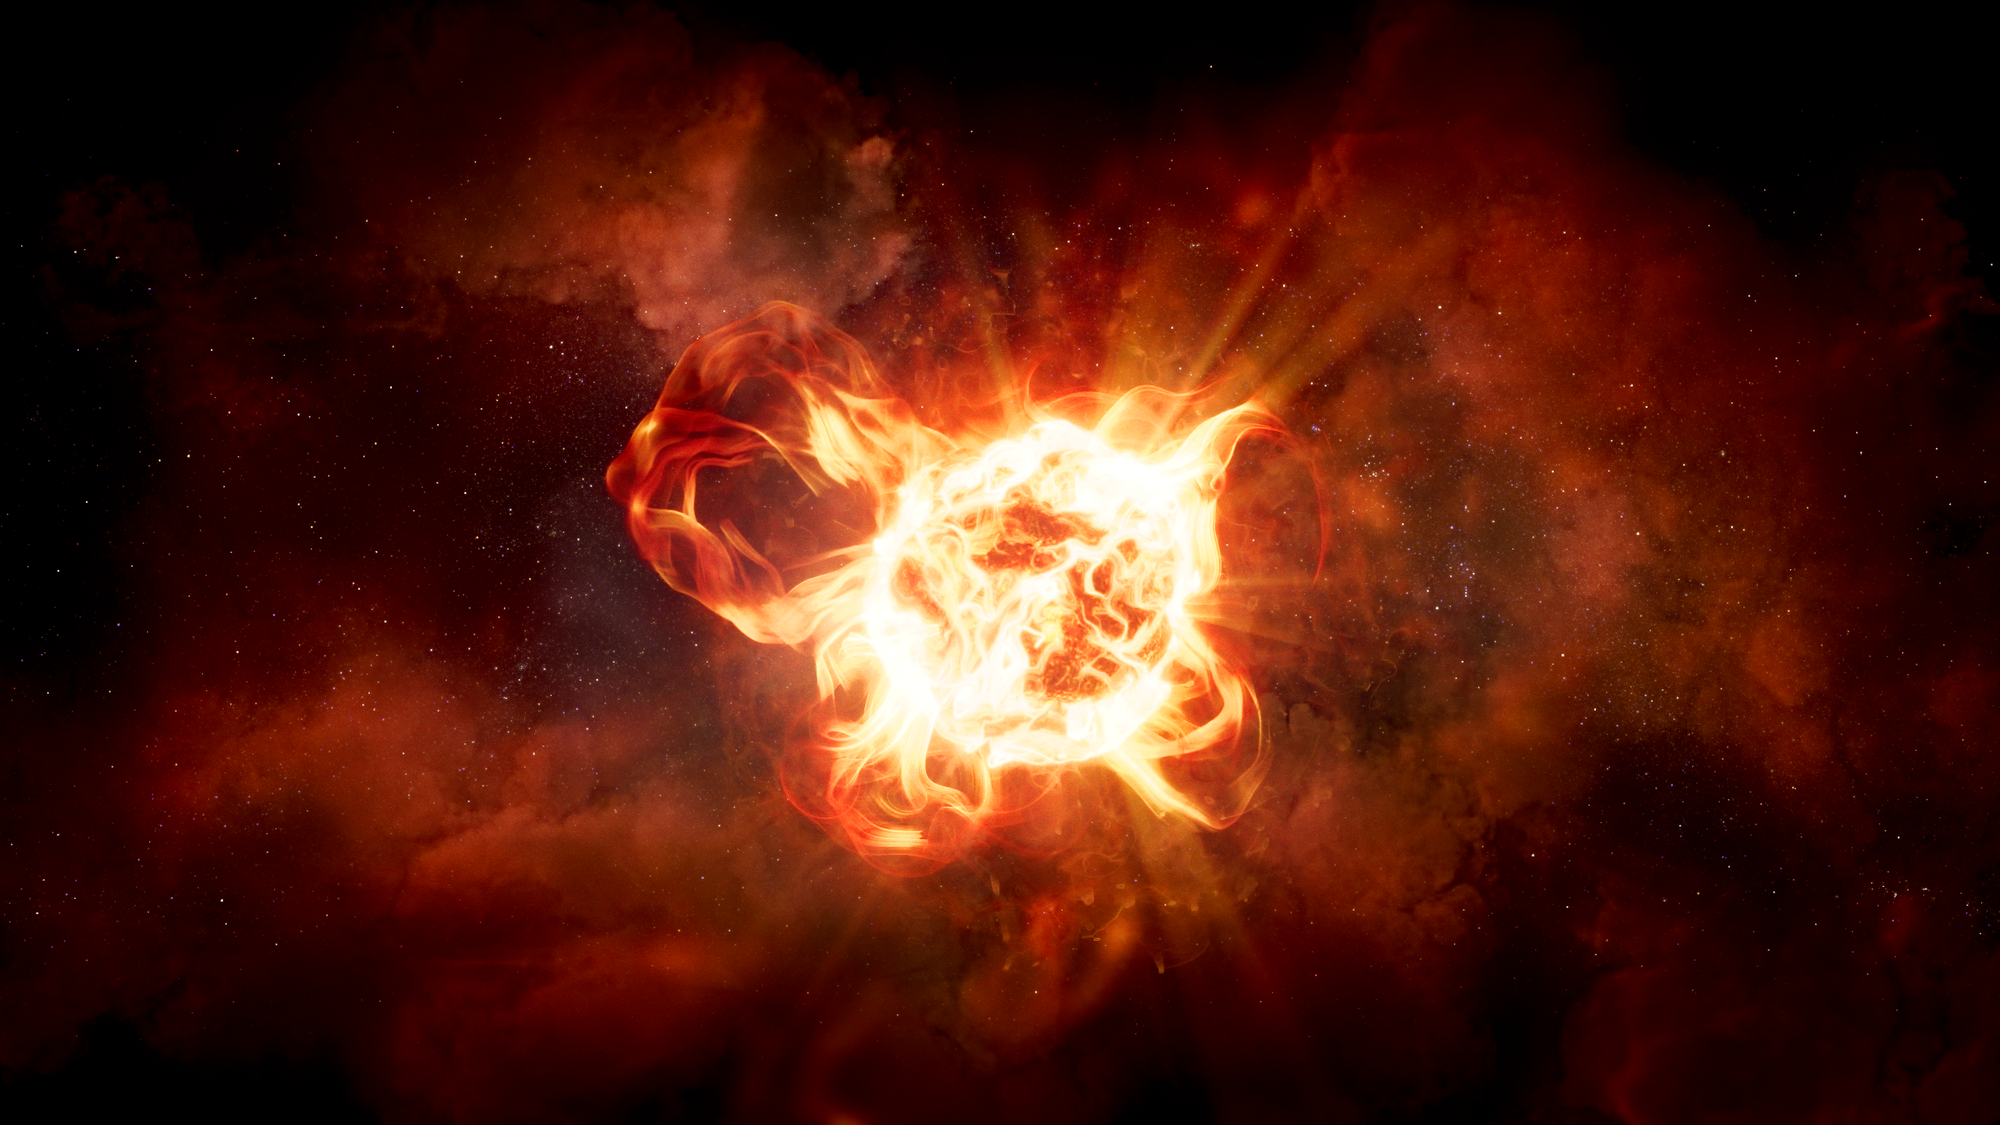
\includegraphics[height=45pt]{figures/stellar_mass_loss.png}};
\end{tikzpicture}
\end{frame}

\begin{frame}{\vspace{-2mm}Horké atmosféry (emise)\phantom{j$^1$}\\\vspace{1.5mm}\hrule}
\vspace{2mm}
\begin{itemize}
    \item<3-> rentgenová emise\\ \vspace{2.4mm}
        -- volně-volné přechody\\ \vspace{2.4mm}
        -- čáry těžkých kovů\\ \vspace{4.5mm}
    \item<5-> ochlazují se vyzařováním\\ \vspace{2.4mm} 
        -- cooling time\\ \vspace{13.5mm}
    \item<7-> vícefázový plyn \\ \vspace{2.4mm}
        -- rentgenový plyn\\ \vspace{2.4mm}
        -- H$\alpha$ filamenty\\ \vspace{4.5mm}
\end{itemize}
\begin{tikzpicture}[overlay]
    % \draw<1-> (10.75, 8.07) node {\includegraphics[height=22pt]{figures/elipsa.png}};

    \draw<2> (1.65,6.1) node {\includegraphics[height=0.33\linewidth]{figures/NGC1275.png}};
    \draw<2> (-0.10,7.65) node[right] {\color{white}Perseus};
    \draw<2> (5.65,6.1) node {\includegraphics[height=0.33\linewidth]{figures/NGC4374.png}};
    \draw<2> (4.00,7.65) node[right] {\color{white}M84};
    \draw<2> (9.75,6.1) node {\includegraphics[height=0.33\linewidth]{figures/NGC4486.png}};
    \draw<2> (7.90,7.65) node[right] {\color{white}M87};
    \draw<2> (1.65,2.3) node {\includegraphics[height=0.33\linewidth]{figures/NGC4552.png}};
    \draw<2> (-0.10,3.85) node[right] {\color{white}M89};
    \draw<2> (5.65,2.3) node {\includegraphics[height=0.33\linewidth]{figures/NGC4636.png}};
    \draw<2> (3.90,3.85) node[right] {\color{white}Centaurus};
    \draw<2> (9.75,2.3) node {\includegraphics[height=0.33\linewidth]{figures/NGC5813.png}};
    \draw<2> (8.00,3.85) node[right] {\color{white}NGC5813};

    % \draw<1-> (10.75, 8.55) node {\includegraphics[height=22pt]{figures/elipsa.png}};

    \draw<4> (8.7, 4.15) node {\includegraphics[height=200pt]{figures/together7.png}};
    \draw<4> (8.65, 4.15) node {\includegraphics[height=200pt]{figures/together3.png}};
    \draw<4> (8.8, 4.15) node {\includegraphics[height=200pt]{figures/together2.png}};
    \draw<4> (8.7, 4.15) node {\includegraphics[height=200pt]{figures/together4.png}};
    \draw<4> (8.7, 4.15) node {\includegraphics[height=200pt]{figures/together5.png}};
    \draw<4> (8.7, 4.15) node {\includegraphics[height=200pt]{figures/together7.png}};

    % % COOLING TIME
    \draw<5-> (3.7, 3.4) node[left] {\Large $t_{\text{cool}} = \frac{3}{2} \frac{n kT}{n_{\text{e}} n_{\text{i}} \Lambda (T, Z)}$};
    \draw<5-> (4.85, 3.4) node[left] {\Large $\propto \frac{kT}{\rho \, \Lambda}$};
    \draw<5-6> (8.2, 5.95) node {\includegraphics[height=110pt]{plots/NGC4472_t_cool.pdf}};
    \draw<6> (6.6, 2.30) node {\includegraphics[height=83pt]{figures/NGC1399_black.png}};
    \draw<6> (8.32, 2.30) node {\includegraphics[angle=90,height=82pt]{figures/NGC1399_scale.png}};
    \draw<6> (10.1, 2.30) node {\includegraphics[height=83pt]{figures/NGC4472_black.png}};

    % % MULTIPHASE GAS
    \draw<7> (7.9, 6.05) node {\includegraphics[height=100pt]{figures/NGC5044.jpg}};
    % \draw<6> (7.9, 2.45) node {\tiny NGC5044, Credit: Werner et al. 2014};
    \draw<7> (7.9, 2.4) node {\includegraphics[height=100pt]{figures/perseus_both.jpg}};
    % \draw<6> (7.9, -1.45) node {\tiny NGC1275, Credit: NASA, ESA};
    \draw<7> (4.17, 1.75) node {({\color{myblue}\textit{modrá}})};
    \draw<7> (3.76, 1.035) node {({\color{red}\textit{červená}})};
\end{tikzpicture}
\end{frame}

\section{Aktivní galaktická jádra}

\begin{frame}{\vspace{-2mm}Aktivní galaktická jádra\phantom{j$^1$}\\\vspace{1.5mm}\hrule}
\vspace{-10.0mm}
\begin{itemize}
    \item<2-> enormní zářivost\\ \vspace{1.5mm} 
        -- $L \approx 10^{10} - 10^{14} \; L_{\odot}$ \\ \vspace{2.1mm}
    \item<2-> netermální spektrum\\ \vspace{2.1mm}
    \item<3-> široké emisní čáry\\ \vspace{1.5mm}
        -- rychlosti $\approx 1000\;$ km\,/\,s\\ \vspace{2.1mm}
    \item<4-> rychlé změny jasnosti\\ \vspace{1.5mm}
        $\Rightarrow$ rozměry $< 1\,$pc\\
\end{itemize}
\begin{tikzpicture}[overlay]
    % \draw<1-> (10.75, 7.1) node {\includegraphics[width=34pt]{figures/AGN.png}};

    \draw<2-> (8.4, 3.4) node {\includegraphics[scale=0.19]{figures/spectral_distribution.png}};
    \draw<3-> (8.90, -0.10) node {\includegraphics[scale=0.12]{figures/emission_lines.png}};
    \draw<4-> (3.0, -0.90) node {\includegraphics[scale=0.11]{figures/lightcurve.png}};
    \draw<2-> (8.4, 5.2) node {\tiny P. Schneider: Extragalactic Astronomy};
\end{tikzpicture}
\end{frame}
% U klasických galaxií naprostá většina světla, které pozorujeme, pochází z hvězd. Jak jistě víte hvězdy září hlavně v infračervené, optické a UV oblasti v závislosti na jejich spektrální třídě, a jejich světlo je víceméně blízké záření absolutně černého tělesa. Takže záření klasické galaxie bude vypadat jako složenina takových absolutně černých zářičů. Navíc v klasických galaxiích máme asi jednu až 10 miliard hvězd, takže zářivý výkon takové galaxie bude přibližně nějakých 10^9 až 10^10 zářivých výkonů Slunce. 

% Existují ale i jiné galaxie, takzvané aktivní galaxie, a tyto galaxie mají řádově vyšší zářivé výkony - asi 10^10 až 10^15 Sluncí, což by v krajním případě odpovídalo až biliardě hvězd. A jejich spektrum se také výrazně liší od spektra klasických galaxií. Spektrum aktivních galaxií je mnohem širší - tyto galaxie vyzařují v celém oboru spektra od radia, přes IR, optickou a UV oblast až po rentgenové nebo dokonce gamma záření. A takové záření je z velké části logicky netermálního původu - určitě by se nedalo popsat jako superpozice absolutně černých zářičů. Zdrojem takového záření tedy pravděpodobně nebudou hvězdy.

% Když se navíc zaměříme na tu optickou oblast aktivních galaxií tak zde také často pozorujeme velmi silné a silně rozšířené emisní čáry. Za předpokladu doplerovského rozšíření čas, ty šířky čar odpovídají rychlostem přesahujícím 1000 km/s. Což je řádově vyšší než běžné rychlosti hvězd v galaxiích.

% A dále záření z těchto galaxií navíc také vykazuje poměrně rychlé změny, v řádu dní až měsíců. A aby se tak rychlé změny stihli projevit v celém objemu takového zdroje, tak to znamená, že ve srovnání s velikostí celé galaxie, ten zdroj tohoto záření musí být poměrně malý. Řádově třeba méně než 1 parsek.

% Máme tedy něco co je poměrně malé, přezáří to celou galaxii, vyzařuj to netermálně v celé oblasti spektra, a plyn se zde pohybuje rychlostmi vyššími než 1000 km/s. Jak asi tušíte, zdrojem takového záření nemůže být nic jiného než supermasivní černá díra neboli aktivní galaktické jádro.

\begin{frame}{\vspace{-2mm}Supermasivní černá díra\phantom{j$^1$}\\\vspace{1.5mm}\hrule}
\vspace{4mm}
\begin{itemize}
    \item<2-> vznikly srážkami a akrecí plynu\\ \vspace{4.0mm}
    \item<4-> popsána 3 parametry:\\ \vspace{3.0mm}
        --  hmotnost $\;\; M_{\bullet} = 10^5 - 10^{10} \; M_{\odot}$\\ \vspace{3.0mm}
        --  spin $\;\; a = \frac{J \, c}{G M^2}$ \hspace{4mm} $J < \frac{G M^2}{c}$ \hspace{4mm} $0 \leq a < 1$\\ \vspace{3.0mm}
        --  náboj $\;\; Q = $ ???\\ \vspace{4.0mm}
    \item<6-> Schwarzschildovo řešení ($a = 0$, $Q = 0$)\\ \vspace{3.5mm}
        \phantom{a} $\;\;\; r_{\text{s}} = \frac{2GM}{c^2}$ \hspace{7mm} $r_{\text{s}} = 0.001 - 400$ AU\\ \vspace{4.0mm}
    \item<7-> Kerrovo řešení ($Q = 0$)\\
\end{itemize}
\begin{tikzpicture}[overlay]
    % \draw<1-> (10.75, 7.1) node {\includegraphics[width=34pt]{figures/AGN.png}};
    \draw<1> (5.7, 3.3) node {\includegraphics[width=190pt]{figures/black_hole.png}};
    
    \draw<3> (2.5, 5.3) node {\Large stelární};
    \draw<3> (2.5, 1.3) node {přímý kolaps};
    \draw<3> (2.5, 3.3) node {\includegraphics[height=90pt]{figures/stellar_bh.jpg}};
    \draw<3> (8.5, 5.3) node {\Large supermasivní};
    \draw<3> (8.5, 1.3) node {srážky + akrece};
    \draw<3> (8.5, 3.3) node {\includegraphics[height=90pt]{figures/M87.jpg}};
    
    \draw<5> (5.7, 1.35) node {\includegraphics[height=50pt]{figures/bh_solutions.png}};
    \draw<6-> (9.6, 5.4) node {\includegraphics[width=85pt]{figures/bh_schwarz.png}};
    \draw<7> (9.6, 1.7) node {\includegraphics[width=85pt]{figures/bh_kerr.png}};
\end{tikzpicture}
\end{frame}
% Takže si uděláme malinkou odbočku a řekneme si co to jsou ty supermasivní černé díry. Obecně černá díra je nějaký gravitačně zhroucený objekt, a v určité vzdálenosti je gravitační síla tak silná, že jejímu působení už neunikne ani světlo.

% Můžeme mít takové ty malé "klasické" černé díry, které vznikají když máme horkou hmotnou hvězdu, které dojde palivo, ta vybuchne jako supernova typu 2 a z jejího jádra se stane stelární černá díra. Pak máme ale ty obrovské černé díry, u kterých zatím není přesně jasné jak vznikají, ale předpokládá se, že v vznikali slučováním těchto menších černých děr v centrech galaxií a následně rostly po miliardy let požíráním okolního plynu.

% Taková černá díra se dá popsat pomocí tří parametrů: nejdůležitější je hmotnost - tedy jak moc hmoty se uvnitř nachází. To jde změřit poměrně dobře, z působení na okolní tělesa - například hmotnost černé díry v centru naší Galaxií vědci určili z pohybu blízkých hvězd, a odhadli ji na nějakých 4 miliony hmotnosti slunce.

% Druhým parametrem je tzv. spin - což vyjadřuje jak rychle se černá díra točí. 


\begin{frame}{\vspace{-2mm}Akrece\phantom{j$^1$}\\\vspace{1.5mm}\hrule}
\begin{itemize}
    \item<1-> akrece okolního plynu (plasmy)\\ \vspace{2.7mm}
        -- diferenciální rotace $\rightarrow$ tření\\ \vspace{4.0mm}
    \item<1-> přeměna $E_p$ na $E_k$ a záření\\ \vspace{4.0mm}
    \item<2-> efektivita přeměny hmoty\\ \vspace{2.7mm}
        -- závisí na rotaci (ISCO)\\ \vspace{2.7mm}
        -- nerotující ($6\,\%$), rotující ($40\,\%$)\\ \vspace{2.7mm}
        -- fůze ($< 1\,\%$)\\
\end{itemize}
\begin{tikzpicture}[overlay]
    % \draw<1-> (10.75, 7.1) node {\includegraphics[width=34pt]{figures/AGN.png}};

    \draw<1-2> (8.8, 4.6) node {\includegraphics[width=120pt]{figures/AGN_artist_view.png}};

    \draw<2> (8.8, 1.0) node {\includegraphics[width=120pt]{figures/ISCO.jpg}};
    \draw<3-> (8.8, 2.8) node {\includegraphics[width=144pt]{figures/bh_orbits.png}};
\end{tikzpicture}
\end{frame}

% \begin{frame}{\vspace{-2mm}Akrece (typy)\phantom{j$^1$}\\\vspace{1.5mm}\hrule}
% \vspace{3mm}
% \begin{itemize}
%     \item efektivita závisí na geometrii\\ \vspace{4mm}
%     \item modely akrece\\ \vspace{47mm}
%     \item Eddingtonova luminosita \hspace{5mm} $L_{\text{Edd}} = \frac{4 \pi G M m_{\text{p}} c}{\sigma_{\text{T}}}$  $\dot{m}_{\text{Edd}} = \frac{L_{\text{Edd}}}{\epsilon c^2}$\\
% \end{itemize}
% \begin{tikzpicture}[overlay]
%     % \draw<1-> (10.75, 5.4) node {\includegraphics[width=34pt]{figures/AGN.png}};
%     \draw<2> (2.3, 2.4) node {\includegraphics[height=85pt]{figures/acc_disk.png}};
%     \draw<2> (5.6, 2.4) node {\includegraphics[height=85pt]{figures/acc_torus.png}};
%     \draw<2> (9.0, 2.4) node {\includegraphics[height=85pt]{figures/spherical.png}};
%     \draw<2> (8.5, 5.7) node {\includegraphics[height=85pt]{figures/znajek.jpg}};
% \end{tikzpicture}
% \end{frame}

\begin{frame}{\vspace{-2mm}Rozdělení AGN\phantom{j$^1$}\\\vspace{1.5mm}\hrule}
\phantom{a}
\begin{tikzpicture}[overlay]
    % \draw<1-> (10.65, 3.7) node {\includegraphics[width=34pt]{figures/AGN.png}};

    \draw<1-5> (1.2, 1.4) node[rotate=310] {BL Lac};
    \draw<1-5> (1.2, -0.1) node[rotate=42] {Blazar};
    \draw<1-5> (1.2, -1.6) node[rotate=287] {Quasar};
    \draw<1-5> (1.2, -3.1) node[rotate=333] {Radio galaxy};
    \draw<1-5> (7.6, 0.3) node[rotate=306] {RLQs};    
    \draw<1-5> (7.6, -1.6) node[rotate=68] {RQQs};
    \draw<1-5> (4.5, 2.2) node[rotate=6] {Liner};
    \draw<1-5> (4.5, 1.3) node[rotate=343] {BLRG};
    \draw<1-5> (4.5, 0.3) node[rotate=51] {NLRG};
    \draw<1-5> (4.5, -0.7) node[rotate=319] {Seyfert 2};
    \draw<1-5> (4.5, -1.6) node[rotate=22] {Seyfert 1};
    \draw<1-5> (4.5, -2.6) node[rotate=44] {Seyfert 1.8};
    \draw<1-5> (4.5, -3.5) node[rotate=17] {Seyfert 1.9};
    \draw<1-5> (9.9, 0.7) node[rotate=287] {FR II};
    \draw<1-5> (9.9, -1.4) node[rotate=308] {FR I};
    
    \draw<2-5> (1.2, 2.7) node {zářivý výkon};
    \draw<2-5>[color=white,thick] (1.2,-0.87) ellipse (1.5cm and 3.3cm);

    \draw<3-5> (4.5, 2.8) node {šířka emisních čar};
    \draw<3-5>[color=white,thick] (4.5,-0.87) ellipse (1.5cm and 3.3cm);

    \draw<4-5> (7.6, 2.0) node {radiová jasnost};
    \draw<4-5>[color=white,thick] (7.6,-0.67) ellipse (0.8cm and 2.3cm);

    \draw<5> (9.9, 2.5) node {radiová morfologie};
    \draw<5>[color=white,thick] (9.9,-0.67) ellipse (0.8cm and 2.3cm);

    \draw<6> (5.7, 2.5) node {\Large Unification scheme};
    \draw<6> (5.7, -1.0) node {\includegraphics[height=170pt]{figures/geometrical.png}};
\end{tikzpicture}
\end{frame}

\begin{frame}{\vspace{-2mm}Kvazar nebo Radiová galaxie?\phantom{j$^1$}\\\vspace{1.5mm}\hrule}
\vspace{3mm}
\scriptsize
\begin{tikzpicture}[overlay]
    % \draw<1-> (10.65, 3.7) node {\includegraphics[width=34pt]{figures/AGN.png}};

    \draw (2.7, 2.3) node {\bf \Large Kvazar\phantom{g}};
    \draw (2.35, 1.1) node[right] {$\bullet \;$ opticky tlustý disk};
    \draw (2.35, 0.4) node[right] {$\bullet \;$ zářivě efektivní};
    \draw (2.35, -0.3) node[right] {$\bullet \;$ $10^{-3}-10^{0} \; \dot{m}_{\text{Edd}}$};
    \draw (2.35, -1.8) node[right] {$\bullet \;$ EM záření};
    \draw (2.35, -2.5) node[right] {$\bullet \;$ rádiově slabé};
    \draw (2.35, -3.2) node[right] {$\bullet \;$ všechny typy galaxií};

    \draw (0.9, 0.4) node {\includegraphics[height=75pt]{figures/acc_disk.png}};
    \draw (0.9, -2.6) node {\includegraphics[height=73pt]{figures/wind.png}};
    
    \draw (8.9, 2.3) node {\bf \Large Radiová galaxie\phantom{g}};
    \draw (8.6, 1.1) node[right] {$\bullet \;$ opticky tenký torus};
    \draw (8.6, 0.4) node[right] {$\bullet \;$ zářivě neefektivní};
    \draw (8.6, -0.3) node[right] {$\bullet \;$ $10^{-6}-10^{-4} \; \dot{m}_{\text{Edd}}$};
    \draw (8.6, -1.8) node[right] {$\bullet \;$ relativistické částice};
    \draw (8.6, -2.5) node[right] {$\bullet \;$ rádiově silné};
    \draw (8.6, -3.2) node[right] {$\bullet \;$ galaxie raného type};

    \draw (7.1, 0.4) node {\includegraphics[height=75pt]{figures/acc_torus.png}};
    \draw (7.1, -2.6) node {\includegraphics[height=73pt]{figures/jet.png}};
\end{tikzpicture}
\end{frame}

% \begin{frame}{\vspace{-2mm}Active galactic nuclei (AGN)\\\vspace{1.5mm}\hrule}
% \begin{tikzpicture}[overlay]
%     \draw<1-> (10.85, 2.64) node {\includegraphics[height=25pt]{figures/AGN.png}};
%     \draw<1-> (8.8, -0.25) node {\includegraphics[height=110pt]{figures/AGN_artist_view.png}};
    
%     \draw<2> (2.7, -4.0) node {\includegraphics[height=85pt]{figures/wind.png}};
%     \draw<2> (8.7, -4.0) node {\includegraphics[height=85pt]{figures/jet.png}};
    
%     \draw<3> (1.7, -4.50) node {\includegraphics[height=85pt]{figures/spherical.png}};
%     \draw<3> (6.0, -4.46) node {\includegraphics[height=85pt]{figures/acc_torus.png}};
%     \draw<3> (9.9, -4.46) node {\includegraphics[height=85pt]{figures/acc_disk.png}};
%     \draw<3> (1.7, -2.9) node {\footnotesize spherical accretion};
%     \draw<3> (6.0, -2.9) node {\footnotesize thick disk / torus};
%     \draw<3> (9.9, -2.9) node {\footnotesize thin disk};
%     %     \draw<3> (9.2, -6.3) node[right] {\tiny Schutte 2017};
%     %     \draw<4> (9.0, -3.0) node {\includegraphics[height=100pt]{figures/NGC4261.jpg}};
%     %     \draw<4> (9.0, -4.9) node {\tiny NGC\,4261, L. Ferrarese (HST)};
%     %     % \draw<7> (10.0, -4.8) node {\includegraphics[height=100pt]{figures/polarimetric_M87.jpg}};
%     %     % \draw<7> (10.0, -6.6) node {\tiny M87, EHT Collaboration};
%     %     % \draw<7> (5.7, -2.8) node {\includegraphics[height=105pt]{figures/rotation.jpg}};
%     %     % \draw<7> (5.7, -5.1) node {\tiny STIS HST};
%     %     \draw<4> (9.0, 0.6) node {\includegraphics[height=100pt]{figures/polarimetric_M87.jpg}};
%     %     \draw<4> (9.0, -0.9) node {\tiny M87, EHT Collaboration};
%     %     \draw<4> (2.3, -3.0) node {\includegraphics[height=98pt]{figures/rotation.jpg}};
%     %     \draw<4> (2.3, -5.1) node {\tiny M87, HST FOS};
% \end{tikzpicture}
% \vspace{-19.9mm}
% \begin{itemize}
%     \item<1-> supermassive black hole\\ \vspace{0.9mm}
%         -- accretes ambient material\\ \vspace{0.9mm}
%         -- rest mass $\rightarrow$ energy (40 \%)\\ \vspace{1.9mm}
%     \item<2-> part of energy is expelled\\ \vspace{0.9mm}
%         -- EM radiation (wind)\\ \vspace{0.9mm}
%         -- relativistic particles (jets)\\ \vspace{1.9mm}
%     \item<3-> geometry of accretion flow\\
% \end{itemize}
% \end{frame}

\begin{frame}{\vspace{-2mm}Radiové galaxie\phantom{j$^1$}\\\vspace{1.5mm}\hrule}
\vspace{-11.5mm}
\begin{itemize}
    \item<1-4> nižší svítivost $L = 10^{8} - 10^{10} L_{\odot}$\\ \vspace{2.5mm}
    \item<1-4> výtrysky relativistických částic $P_{\text{jet}} = 10^{10} - 10^{13} L_{\odot}$\\ \vspace{2.5mm}
    \item<1-4> částice (e$^-$, e$^+$) v magnetickém poli\\ \vspace{1.8mm}
        $\Rightarrow$ synchrotronová emise $\Rightarrow$ radiové laloky\\ \vspace{2.5mm}
    \item<3-4> Fanaroff–Riley klasifikace\\ \vspace{2.5mm}
    \item<4> pozorování - VLA, LOFAR, MWA\\
\end{itemize}
\begin{tikzpicture}[overlay]
    % \draw<1-> (10.65, 3.7) node {\includegraphics[width=34pt]{figures/AGN.png}};

    \draw<2> (2.6, -0.40) node {\includegraphics[height=105pt]{figures/synchrotron.pdf}};
    \draw<2> (5.7, -0.40) node {\Large \myarrow[0.25pt]};
    \draw<2> (8.80, -0.40) node {\includegraphics[height=105pt]{figures/hercules_A_flop.png}};

    % \draw<3> (9.20, 3.11) node {\includegraphics[width=55pt]{figures/FRI.png}};
    % \draw<3> (9.20, 5.07) node {FR I};
    % \draw<3> (9.20, -0.66) node {\includegraphics[width=55pt]{figures/FRII.png}};
    % \draw<3> (9.20, 1.08) node {FR II};
    % \draw<3> (3.70, -0.66) node {\includegraphics[width=130pt]{figures/FRI_FRII.png}};

    \draw<3> (2.00, -0.66) node {\includegraphics[height=95pt]{figures/FRI.png}};
    \draw<3> (0.32, -0.52) node {\bf FR I};
    \draw<3> (9.40, -0.66) node {\includegraphics[height=95pt]{figures/FRII.png}};
    \draw<3> (11.10, -0.52) node {\bf FR II};
    \draw<3> (5.70, -0.66) node {\includegraphics[height=95pt]{figures/FRI_FRII.png}};
    
    \draw<4> (1.8, -0.95) node {\includegraphics[height=67pt]{figures/VLA.jpg}};
    \draw<4> (1.8, -2.38) node {\scriptsize $1 - 2$ GHz};
    \draw<4> (5.65, -0.95) node {\includegraphics[height=67pt]{figures/LOFAR.jpg}};
    \draw<4> (5.65, -2.38) node {\scriptsize $10 - 240$ MHz};
    \draw<4> (9.5, -0.95) node {\includegraphics[height=67pt]{figures/MWA.jpg}};
    \draw<4> (9.5, -2.38) node {\scriptsize $70 - 300$ MHz};
    
    \draw<5> (1.75, 3.05) node {\includegraphics[height=120pt]{figures/M87_lobes.png}};
    \draw<5> (5.4, 3.05) node {\includegraphics[height=120pt]{figures/M84_lobes.jpg}};
    \draw<5> (9.35, 3.05) node {\includegraphics[height=120pt]{figures/Fornax_A.jpg}};
    \draw<5> (0.03, 4.87) node[right] {\bf M87};
    \draw<5> (3.77, 4.87) node[right] {\bf M84};
    \draw<5> (7.30, 4.87) node[right] {\bf Fornax A};
    
    \draw<5> (3.65, -0.80) node {\includegraphics[height=90pt]{figures/Cygnus_A_lobes.png}};
    \draw<5> (8.70, -0.80) node {\includegraphics[height=90pt]{figures/Centaurus_A.jpg}};
    \draw<5> (0.90, 0.50) node[right] {\bf Cygnus A};
    \draw<5> (6.65, 0.50) node[right] {\bf Centaurus A};
\end{tikzpicture}
\end{frame}

\section{Zpětná vazba AGN}

\begin{frame}{\vspace{-2mm}Zpětná vazba AGN\phantom{j$^1$}\\\vspace{1.5mm}\hrule}
\vspace{-10mm}
\begin{itemize}
    \item<1-> interakce jetů a atmosfér\\ \vspace{2.2mm}
        $\Rightarrow$ rentgenové dutiny\\ \vspace{3mm}
    \item<3-> ohřev atmosféry\\ \vspace{2.2mm}
        -- zvukové a rázové vlny\\ \vspace{2.3mm}
        -- turbulentní proudění\\ \vspace{2.2mm}
        -- disipace dutin\\ \vspace{3mm}
\end{itemize}
\begin{tikzpicture}[overlay]
    % \draw<1-> (10.65, 5.95) node {\includegraphics[width=19pt]{figures/loby.png}};

    \draw<1-> (8.2, 3.3) node {\includegraphics[height=100pt]{figures/cygnus_A.jpg}};
    \draw<2> (2.9, -0.05) node {\includegraphics[height=115pt]{figures/MS0735.jpg}};
    \draw<2> (8.2, -0.3) node {\includegraphics[height=100pt]{figures/hydra.jpg}};
    \draw<4-> (8.7, -0.8) node {\includegraphics[height=80pt]{figures/perseus_sound_waves.jpg}};
    \draw<5-> (3.7, -0.8) node {\includegraphics[height=80pt]{figures/turbulent_flows.png}};
\end{tikzpicture}
\end{frame}

% \begin{frame}{\vspace{-2mm}Ohřev atmosféry\phantom{j$^1$}\\\vspace{1.5mm}\hrule}
% \begin{itemize}
%     \item způsoby
%     \item 
% \end{itemize}
% \end{frame}

\begin{frame}{\vspace{-2mm}Zpětná vazba (mechanismus)\phantom{j$^1$}\\\vspace{1.5mm}\hrule}
\vspace{-43mm}
\begin{tikzpicture}[overlay]
    % \draw<1-> (10.65, 3.6) node {\includegraphics[width=19pt]{figures/loby.png}};

    % PICTURES
    \draw<8> (2.5, -5.05) node {\includegraphics[scale=0.175]{figures/cold.png}};
    \draw<8> (8.9, -5.2) node {\includegraphics[scale=0.125]{figures/hot.png}};
    \draw<8>[->,line width=0.4mm] (5.21, -4.15) arc (135:45:0.7cm);
    \draw<8>[->,line width=0.4mm] (6.22, -6.18) arc (315:225:0.7cm);

    % CYCLE
    \draw<1-8> (5.6, 0.05) node {\Large Jak se výkon jetů reguluje?};
    \draw<2-8> (1.65, -1.8) node {\begin{tcolorbox}[colback=mycolor,colframe=mycolor,width=24mm,boxsep=-2pt,left=5pt,right=-5pt,arc=6pt]plyn chládne\hspace{-3mm}\phantom{Aj}\end{tcolorbox}};
    \draw<3-8>[->,line width=0.4mm] (2.05, -1.3) arc (180:90:0.5cm);
    \draw<3-8> (4.00, -0.9) node {\begin{tcolorbox}[colback=mycolor,colframe=mycolor,width=27.1mm,boxsep=-2pt,left=5pt,right=-5pt,arc=6pt]padá na SMBH\hspace{-3mm}\phantom{Aj}\end{tcolorbox}};
    \node (A) at (5.40, -0.83) {};
    \node (B) at (6.10, -0.83) {};
    \draw<4-8>[->,line width=0.4mm] {(A) edge (B)};
    \draw<4-8> (7.30, -0.9) node {\begin{tcolorbox}[colback=mycolor,colframe=mycolor,width=22.9mm,boxsep=-2pt,left=5pt,right=-5pt,arc=6pt]aktivuje  jety\hspace{-3mm}\phantom{Aj}\end{tcolorbox}};
    \draw<5-8>[->,line width=0.4mm] (8.78, -0.83) arc (90:0:0.5cm);
    \draw<5-8> (9.77, -1.8) node {\begin{tcolorbox}[colback=mycolor,colframe=mycolor,width=23.4mm,boxsep=-2pt,left=5pt,right=-5pt,arc=6pt]ohřívají plyn\hspace{-3mm}\phantom{Aj}\end{tcolorbox}};
    \draw<6-8>[->,line width=0.4mm] (9.30, -2.25) arc (360:270:0.5cm);
    \draw<6-8> (7.30, -2.7) node {\begin{tcolorbox}[colback=mycolor,colframe=mycolor,width=27.2mm,boxsep=-2pt,left=5pt,right=-5pt,arc=6pt]omezuje akreci\hspace{-3mm}\phantom{Aj}\end{tcolorbox}};
    \node (A) at (6.00, -2.75) {};
    \node (B) at (5.30, -2.75) {};
    \draw<7-8>[->,line width=0.4mm] {(A) edge (B)};
    \draw<7-8> (4.0, -2.7) node {\begin{tcolorbox}[colback=mycolor,colframe=mycolor,width=26.9mm,boxsep=-2pt,left=5pt,right=-5pt,arc=6pt]deaktivuje jety\hspace{-3mm}\phantom{Aj}\end{tcolorbox}};
    \draw<7-8>[->,line width=0.4mm] (2.55, -2.75) arc (270:180:0.5cm);
\end{tikzpicture}
\end{frame}

\begin{frame}{\vspace{-2mm}Důsledky mechanické zpětné vazby\phantom{j$^1$}\\\vspace{1.5mm}\hrule}
\vspace{-16mm}
\begin{tikzpicture}[overlay]
    % \draw<1-> (10.65, 2.8) node {\includegraphics[width=19pt]{figures/loby.png}};

    \draw<1-> (5.7, 1.5) node {\Large přijatá $E$ $\approx$ vyzářená $E$};
    \draw<2-> (3.0, 0.7) node {horká atmosféra};
    \draw<3-> (8.4, 0.7) node {aktivní galaktické jádro};
    \draw<2-> (3.0, -2.20) node {\includegraphics[width=135pt]{figures/cooling_luminosity.png}};
    \draw<3> (8.4, -2.20) node {\includegraphics[width=135pt]{figures/allen.pdf}};
    \draw<4-> (8.4, -2.20) node {\includegraphics[width=135pt]{figures/russel.pdf}};
\end{tikzpicture}
\end{frame}

\begin{frame}{\vspace{-2mm}Vliv na tvorbu hvězd\phantom{j$^1$}\\\vspace{1.5mm}\hrule}
\vspace{-30mm}
\begin{itemize}
    \item atmosféra nechládne $\Rightarrow$ potlačena tvorba hvězd\\ \vspace{3mm}
    \item hmotnější galaxie $\Rightarrow$ silnější AGN\\
\end{itemize}
\begin{tikzpicture}[overlay]
    % \draw<1-> (10.65, 2.85) node {\includegraphics[width=19pt]{figures/loby.png}};

    \draw<2> (5.7, -2.45) node {\includegraphics[height=155pt]{figures/SFR.png}};
\end{tikzpicture}
\end{frame}

\section{Cavity Detection Tool}

\begin{frame}{\vspace{-2mm}Cavity Detection Tool - motivace\phantom{j$^1$}\\\vspace{1.5mm}\hrule}
\begin{tikzpicture}[overlay]
    % \draw<1-> (10.85, 3.705) node {\includegraphics[height=25pt]{figures/blackcadet.png}};
    \draw<1-> (3.4, -0.6) node {\includegraphics[width=190pt]{CADET/NGC5813.jpeg}};
    \draw<1-> (1.25, 2.25) node {\large NGC5813};
    \draw<2-6> (8.9, 1.15) node {\includegraphics[width=105pt]{CADET/NGC4778.png}};
    \draw<2-6> (8.05, 2.65) node {\normalsize NGC4778};
    \draw<5-6> (8.9, -2.7) node {\includegraphics[width=105pt]{CADET/NGC4649.png}};
    \draw<5-6> (8.05, -1.2) node {\normalsize NGC4649};
    \draw<3-6>[rotate=30,color=green,line width=0.8pt] (8.27, -2.9) ellipse (0.3cm and 0.22cm);
    \draw<3-6>[rotate=35,color=green,line width=0.8pt] (7.85, -4.85) ellipse (0.19cm and 0.17cm);
    \draw<4-6>[rotate=36,color=yellow,line width=0.8pt] (7.93, -3.75) ellipse (0.26cm and 0.27cm);
    \draw<4-6>[rotate=28,color=yellow,line width=0.8pt] (8.36, -3.85) ellipse (0.235cm and 0.16cm);
    % \draw<4-6>[rotate=30,color=green,line width=0.8pt] (1.72, -1.0) ellipse (0.6cm and 0.45cm);
    % \draw<4-6>[rotate=35,color=green,line width=0.8pt] (1.5, -3.0) ellipse (0.38cm and 0.33cm);
    % \draw<5-6>[rotate=36,color=yellow,line width=0.8pt] (1.63, -1.2) ellipse (0.54cm and 0.49cm);
    % \draw<5-6>[rotate=28,color=yellow,line width=0.8pt] (1.85, -2.75) ellipse (0.45cm and 0.30cm);
    \draw<6> (9.0, -2.5) node {\color{green}\Huge\selectfont ?};
\end{tikzpicture}
\end{frame}


\begin{frame}{\vspace{-2mm}Cavity Detection Tool\phantom{j$^1$}\\\vspace{1.5mm}\hrule}
\vspace{-18.5mm}
\begin{itemize}
    \item<1-> umělé vytvořené snímky\\ \vspace{1.0mm}
        -- 300 tisíc snímků \\ \vspace{1.0mm}
        -- 50\,\% bez dutin\\ \vspace{2.1mm}
    \item<2-> CADET architektura\\ \vspace{1.0mm}
        -- 5 konvolučních bloků\\ \vspace{1.0mm}
        -- clusterovací algoritmus 
\end{itemize}
\begin{tikzpicture}[overlay]
    % \draw<1-> (10.85, 4.84) node {\includegraphics[height=25pt]{figures/blackcadet.png}};
    \draw<2-> (8.6, 3.46) node {\includegraphics[height=35pt]{CADET/nothing.png}};
    \draw<2-> (8.6, 2.21) node {\includegraphics[height=35pt]{CADET/cavities.png}};
    \draw<2-> (8.6, 0.96) node {\includegraphics[height=35pt]{CADET/all.png}};
    \draw<3-> (5.7, -1.45) node {\includegraphics[width=320pt]{CADET/blocks.png}};
\end{tikzpicture}
\end{frame}
% Pro přesnější a nezaujaté hledání a určování velikostí dutin jsem tedy vytvořil a natrénoval neuronovou síť, kterou jsem pracovně nazval CADET neboli CAvity DEtection Tool.

% Pro trénování této sítě jsem nepoužil reálné snímky. Místo toho jsem uměle vygeneroval dostatečně velkou trénovací sadu takovýchto umělých snímků různých galaxií do nichž jsem náhodně vkládal různě velké dutiny. A přidal jsem i další typické rysy, jsou jsou například jasné bodové zdroje v centru, jasné okraje dutin nebo případně nějaké antisymetrické poruchy, aby se ty uměle vytvořené snímky co nejvíce podobaly reálným snímkům z observatoře Chandra.

% Ta samotná síť se skládá z konvoluční neuronové sítě a z klastrovacího algoritmu DBSCAN. A úkolem této konvoluční neuronové sítě je, z takovéhoto původního snímku, vytvořit predikci, kde na snímku se tyto dutiny nacházejí. Hodnota každého pixelu vyjadřuje pravděpodobnost, že ten daný pixel je součástí dutiny. A na tuto predikci je následně aplikován klastrovací algoritmus, který provede dekompozici této predikce na jednotlivé dutiny. A pro takto získané dutiny my můžeme následně, opět za pomocí nějakých zjednodušujících předpokladů, určit jejich velikosti.

\begin{frame}{\vspace{-2mm}Cavity Detection Tool - výsledky\phantom{j$^1$}\\\vspace{1.5mm}\hrule}
\begin{tikzpicture}[overlay]
    % \draw<1-> (10.85, 3.68) node {\includegraphics[height=25pt]{figures/blackcadet.png}};
    \draw<1> (3.3, 1.18) node {\includegraphics[height=137pt]{CADET/NGC5813_CNN.pdf}};
    \draw<1> (7.95, 1.18) node {\includegraphics[height=137pt]{CADET/NGC4649_CNN.pdf}};
    \draw<1> (3.3, -2.74) node {\includegraphics[height=137pt]{CADET/NGC4778_CNN.pdf}};
    \draw<1> (7.95, -2.74) node {\includegraphics[height=137pt]{CADET/NGC6166_CNN.pdf}};
\end{tikzpicture}
\end{frame}
% Nyní si tedy ukážeme využití té neuronové sítě na reálné snímky galaxií. Zde vidíme tedy víceméně surový snímek galaxie z té rentgenové observatoře Chandra. 

\begin{frame}{\vspace{-2mm}Korelace\phantom{j$^1$}\\\vspace{1.5mm}\hrule}
\begin{tikzpicture}[overlay]
    % \draw<1-> (10.85, 3.68) node {\includegraphics[height=25pt]{figures/blackcadet.png}};

    \draw<1> (5.7, -0.6) node {\includegraphics[height=165pt]{figures/PBondi_Pjet_radio.pdf}};

    \draw<2> (2.8, -0.6) node {\includegraphics[height=145pt]{figures/M_BH-jet_power.pdf}};
    \draw<2> (8.6, -0.6) node {\includegraphics[height=145pt]{figures/MBH_Pjet_CADET.pdf}};
\end{tikzpicture}
\end{frame}

\begin{frame}[noframenumbering,plain]
\begin{tikzpicture}[overlay]
    \draw (5.67, -0.8) node {\includegraphics[scale=0.5]{figures/meme.jpg}};
\end{tikzpicture}
\end{frame}

\end{document}
